\subsection{Leiter des Turnverein-Orchesters}

\hypertarget{RefHeadingToc100333730}{}Ähnlich wie andere Vereine am Ort,
veranstaltete der Turnverein Ruhmannsfelden bunte Abende oder führte
Theaterstücke, Singspiele und sogar Operetten auf und übernahm somit
weit über die eigentliche Vereinsaufgabe hinaus eine wichtige
kulturelle Funktion. \footnote{Dokument Nr. 56, Auszug aus den Memoiren
von Franz Danziger sen., 1984} Zumindest für den Turnverein war die
Veranstaltung derartiger Unterhaltungsprogramme eine bedeutende
Einnahmequelle für die Finanzierung geplanter Projekte wie
beispielsweise den Turnhallenbau. Es ist daher keineswegs
verwunderlich, dass sich für August Högn in den Anfangsjahren in
Ruhmannsfelden insbesondere unter dem Dach des Turnvereins ein
musikalisches Betätigungsfeld auftat, obwohl die ursprüngliche Aufgabe
des Vereins nichts mit Musik zu tun hatte. Der ehemalige Vorstand
unterstützte den Verein nun als Leiter einer Sänger- und
Orchesterriege. \footnote{Dokument Nr. 98, Geschichtliches über die
Erbauung der Turnhalle in Ruhmannsfelden, 1928}

Am 27.9.1919 wurde die Sängerriege im Turnverein gegründet. Als erster
Leiter erscheint zwar Rudolf Schwannberger, Nachbar von Högn und
Kirchenchorsänger. \footnote{Dokument Nr. 104, Protokoll der
Turnvereinsversammlung, 27.9.1919} Doch laut des Turnverein-Protokolls
fungierte Högn bereits ab 29.12.1919 als Dirigent. \footnote{Dokument
Nr. 105, Protokoll der Turnvereinsversammlung, 29.12.1919} 1921 wird
Schwannberger als Gesangswart und Högn als Gesangsdirigent der
Sängerriege bezeichnet, \footnote{Dokument Nr. 106, Protokoll der
Turnvereinsversammlung, 10.12.1921} die sich im Saal der Brauerei
Vornehm zum Proben traf. Über die Orchesterriege, die im Haus des
Apothekers Voit probte, sind im Vereinsprotokoll keine Eintragungen zu
finden. Wahrscheinlich kam das Streichorchester nur dann zusammen, wenn
ein Stück eine Instrumentalbegleitung der Sänger benötigte.

\begin{center}
\begin{minipage}{6.682cm}
\begin{flushleft}
\tablefirsthead{}
\tablehead{}
\tabletail{}
\tablelasttail{}
\begin{supertabular}{m{3.1069999cm}m{3.174cm}}

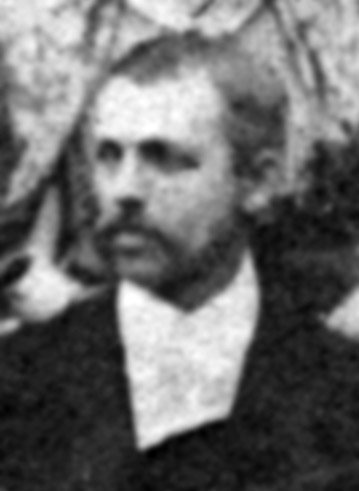
\includegraphics[width=2.925cm,height=4.001cm]{pictures/zulassungsarbeit-img019.jpg}

Abb. \stepcounter{Abb}{\theAbb}: August Högn &

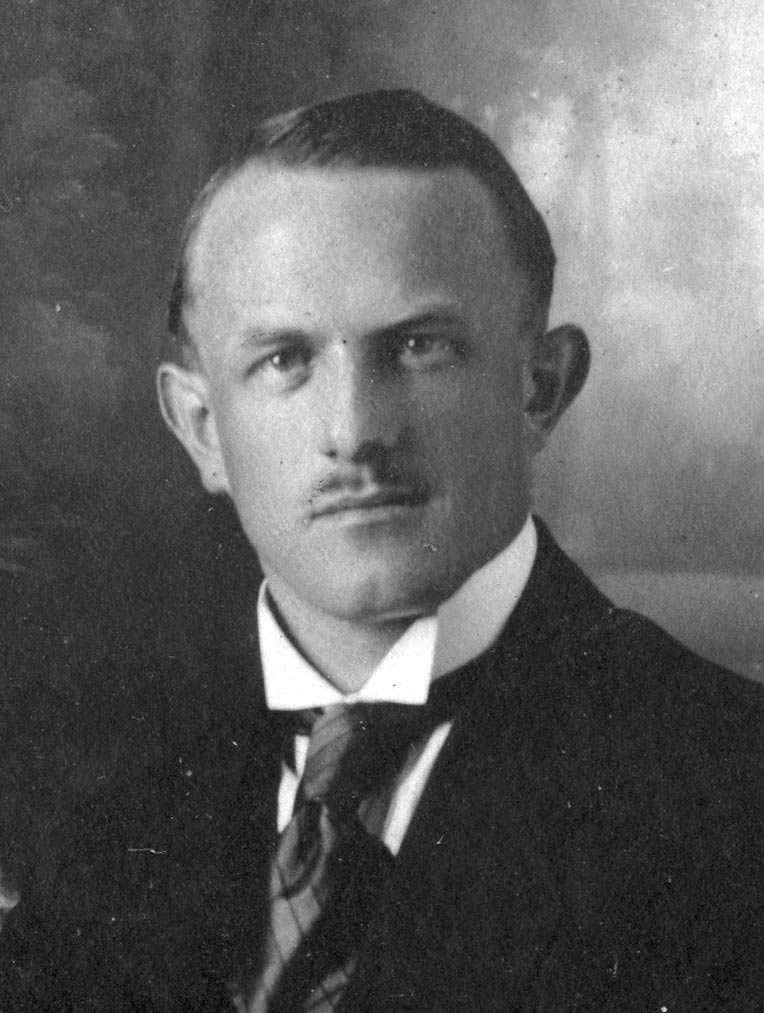
\includegraphics[width=2.992cm,height=3.993cm]{pictures/zulassungsarbeit-img020.jpg}

Abb. \stepcounter{Abb}{\theAbb}: Rudolf Schwannberger\\
\end{supertabular}
\end{flushleft}
\end{minipage}
\end{center}
Leider ist nur wenig über die Veranstaltungen im Einzelnen bekannt. Es
ist nicht bekannt, wie regelmäßig sie stattfanden und in welchem
Zeitraum der Turnverein sich derart kulturell engagierte. Einen kleinen
Einblick in das damalige kulturelle Leben gewährt uns aber, die nicht
nur in finanzieller Hinsicht erfolgreichste „Produktion“ des
Turnvereins: die Aufführungen des Singspiels „Der Holledauer Fidel“ von
Erhard Kutschenreuter im Jahr 1923. \footnote{Dokument Nr. 98,
Geschichtliches über die Erbauung der Turnhalle in Ruhmannsfelden,
1928} Dieses Singspiel forderte eine große Anzahl an Mitwirkenden. Im
dritten Akt ist beispielsweise ein Trachtenfestzug verlangt, der über
die Bühne zieht. \footnote{Proft, Seite 58} Große Anforderungen an die
Gesangeskünste der Mitwirkenden stellten die vielen Gesangsnummer des
Singspiels, wie etwa das Liebeslied des Fidel, das Duett des Sichbauern
und dessen Frau, das Lied der Reserl, ein Kinderchor und die großen
Chorszenen zu Beginn und zum Schluss des Singspiels. \footnote{Proft,
Seite 57} Instrumentalstücke, wie zum Beispiel das polyphon angelegt
Vorspiel zum zweiten Akt \footnote{Proft, Seite 55} der
„Holledauer-Marsch“ und der „Waldler-Marsch“, \footnote{Proft, Seite
57} stellten eine Herausforderung für das Turnverein-Orchester dar, das
aus drei Violinen und einer Viola, einem Violoncello und einem
Kontrabass, also sechs Musikern, ähnlich wie das Kirchenorchester,
bestand.


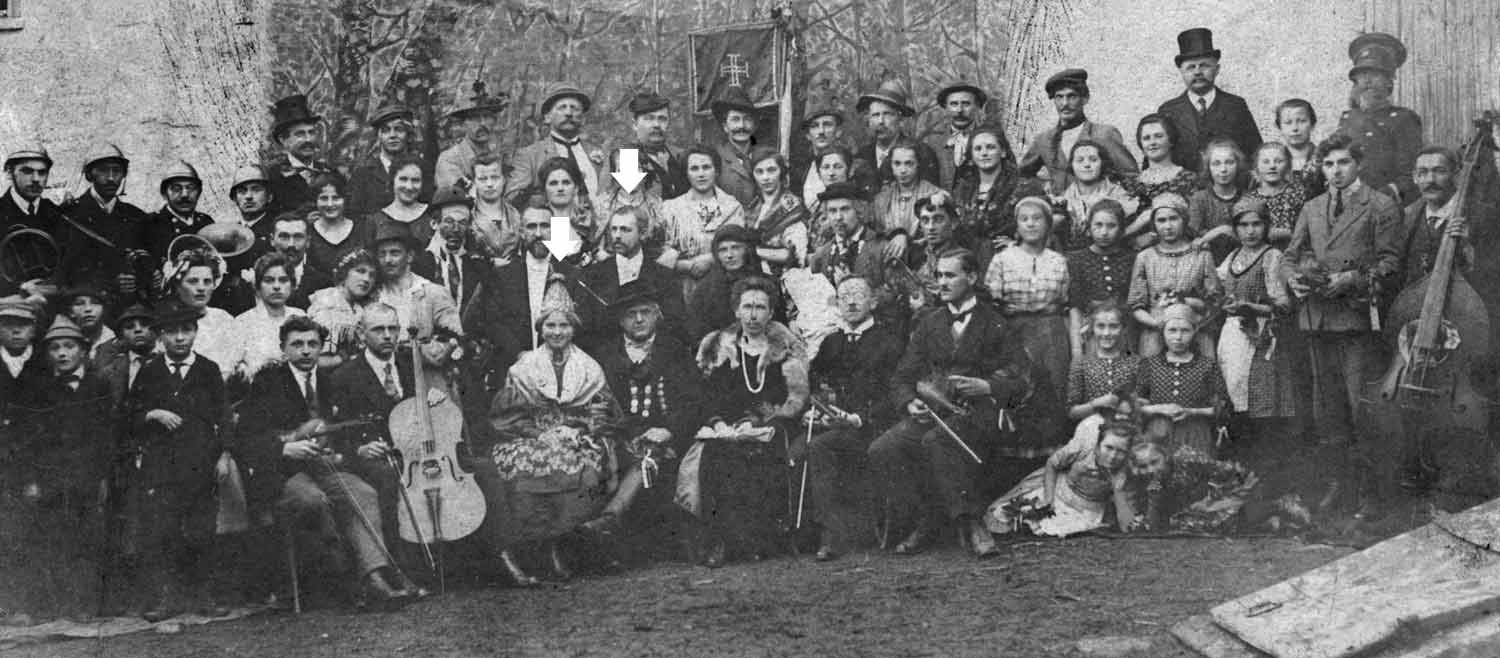
\includegraphics[width=15.993cm,height=7.015cm]{pictures/zulassungsarbeit-img021.jpg}


\label{bkm:Ref100050511}Abb. \stepcounter{Abb}{\theAbb}: Die ca. 60 an
den 8 Aufführungen des Singsspiels „Der Holledauer Fidel“ von Erhard
Kutschenreuter im März 1923 beteiligten Personen. In der Mitte (Pfeile)
sind August Högn und seine Tochter Frieda zu sehen.

Diese ungewöhnlich große Anzahl an Mitwirkenden – auf dem Foto (Abb. 19)
sind 60 Personen zu sehen – machte es notwendig, dass die Bühne im
Vornehmsaal ausnahmsweise an der Längsseite aufgestellt werden musste,
sodass die Akteure nur direkt vom Freien aus auf die Bühne gelangen
konnten. \footnote{Dokument Nr. 98, Geschichtliches über die Erbauung
der Turnhalle in Ruhmannsfelden, 1928} Die große Teilnehmerzahl ist auf
die Unterstützung weiterer Vereine zurückzuführen, insbesondere jedoch
des Kirchenchores und der Lehrerschaft. August Högn, der die gesamte
musikalische Leitung übernommen hatte und als Dirigent fungierte, war
in seiner Eigenschaft als Chorregent und Schulleiter der ideale Mann,
weitere geeignete Mitwirkende für das Singspiel zu gewinnen.

Die Einkünfte der acht im Saal der Brauerei Vornehm stattgefundenen und
ausverkauften Aufführungen des Singspiels erbrachten einen Gewinn von
500 M, mit dem ein Grundstück erworben werden konnte, das als Turnplatz
verwendet wurde. \footnote{Dokument Nr. 95, Programmzettel zur
Aufführung des Singspiels {\textquotedbl}Der Holledauer
Fidel{\textquotedbl}, Mrz. 1923} Dieser durchschlagende Erfolg der
Aufführungen des „Fidels“ – sie verhalfen dem Turnverein sogar zu einem
eigenen Turnplatz – ist auch auf das Stück zurückzuführen. Mit dem
„Fidel“ hatte der im Rottal ansässige Lehrer Erhard Kutschenreuter mit
Abstand sein erfolgreichstes Stück geschrieben. \footnote{Proft, Seite
53} Nach der Uraufführung in Passau im Jahr 1920 erlebte das Singspiel
schon 1938 die 3000. Aufführung. \footnote{Proft, Seite 60} Die
Ruhmannsfeldener Zuschauer strömten vielleicht auch deswegen so
zahlreich in die Vorstellungen weil die Handlung des Stückes zum Teil
im bayerischen Wald spielt: Der arme Hopfenzupfer Fidel Waldhauser aus
dem bayerischen Wald verliebt sich in die Tochter des reichen
Sichbauern aus der Hallertau, gespielt von August Högns Tochter
Frieda. \footnote{Dokument Nr. 95, Programmzettel zur Aufführung des
Singspiels {\textquotedbl}Der Holledauer Fidel{\textquotedbl}, Mrz.
1923} Trotz auftretender Hindernisse, die unüberwindbar zu sein
scheinen, findet das ungleiche Paar schließlich doch zusammen, und es
kommt zur Hochzeit. Den Zuschauern in Ruhmannsfelden waren die
dargestellten sozialen Verhältnisse sicher gut bekannt, denn viele von
ihnen fuhren selbst, wie es bis in den fünfziger Jahren des letzten
Jahrhundert üblich war, einmal jährlich in die Hallertau zur
Hopfenernte, um ein Zusatzeinkommen zu verdienen. \footnote{Proft,
Seite 56}

\begin{center}
\begin{minipage}{5.794cm}
\begin{center}
\tablefirsthead{}
\tablehead{}
\tabletail{}
\tablelasttail{}
\begin{supertabular}{m{5.5940003cm}}

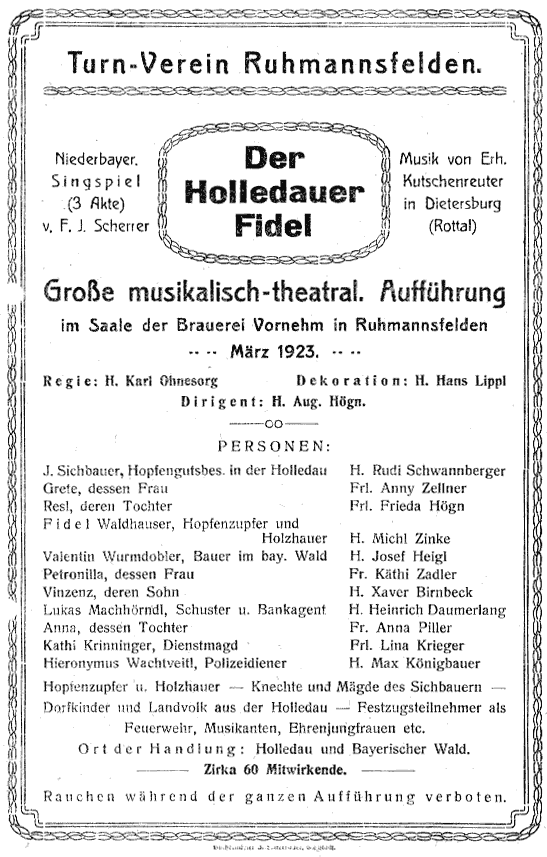
\includegraphics[width=5.412cm,height=8.456cm]{pictures/zulassungsarbeit-img022.png}

Abb. \stepcounter{Abb}{\theAbb}: Programm zu den „Fidel“-Aufführungen\\
\end{supertabular}
\end{center}
\end{minipage}
\end{center}
Am 21. Juli 1923 wurde August Högn von der Gemeinde Ruhmannsfelden das
Ehrenbürgerrecht \zitat{„aus Anlass seines 25-jährigen
Dienstjubiläums“ }\footnote{Reicheneder-Chronik, Ehrenbürger, Blatt 1
Vorderseite} und \zitat{„für die großen Verdienste, die er
sich um Schule und Gemeinde erwarb“ }\footnote{Reicheneder-Chronik, Ehrenbürger, Blatt 1
Vorderseite} verliehen. Dieser Titel stellte damals schon eine
besondere Auszeichnung dar und wurde daher nur an wenige sich
außerordentlich verdient gemachte Bürger verliehen. Die
Ehrenbürgerurkunde bekamen außerdem Pfarrer Mühlbauer (1906) sowie
August Högns Vorgänger als Schulleiter Alois Auer (1910). Nach Högn
wurde sie 1933 an Adolf Hitler verliehen.\footnote{Reicheneder-Chronik, Ehrenbürger, Blatt 1
Vorderseite} Die Aufführungen des „Holledauer Fidels“ etwas länger als
ein Vierteljahr davor, lassen den Anlass für die
Ehrenbürgerrechts-Verleihung Högns in ganz anderem Licht erscheinen.
Ist es nicht offensichtlich, dass die Singspielabende, an denen Högn in
hervorragender Weise mitgearbeitet hatte und die dem Turnverein zum
Erwerb eines Turnplatzes verhalfen, eher als der Hauptgrund für die
Verleihung anzusehen ist, als sein 25. Dienstjubiläum, das wohl eher
einen weiterem Grund darstellt?

Aus finanzieller Sicht war der Turnverein am Bau seiner eigenen
Turnhalle mit einem großen Betrag beteiligt. Die Einkünfte vieler
bunter Abende sowie weitere Theateraufführungen, wie z. B. die
Aufführung der Operette „Der Postillion“  \footnote{Dokument Nr. 56,
Auszug aus den Memoiren von Franz Danziger sen., 1984} von Ludwig
Eckl, \footnote{Goller, Seite 188} dürften direkt in den Turnhallenbau
geflossen sein. Högn engagierte sich nicht nur musikalisch für die
Anliegen des Turnvereins, sondern auch politisch. 1925 begrüßte er eine
Kommission des bayerischen Landtages in Ruhmannsfelden und äußerte
ihnen unter anderem die Bitte um Bezuschussung des Turnhallenbaus. Am
29. Januar 1928 wurde die Ruhmannsfeldener Turnhalle schließlich
eingeweiht und ein \zitat{„großers Orchester aus lauter
Ruhmannsfeldener Musikern“ } \footnote{Dokument Nr. 98, Geschichtliches
über die Erbauung der Turnhalle in Ruhmannsfelden, 1928} spielte zur
Feier des Tages.

\begin{center}
\begin{minipage}{9.684cm}
\begin{flushleft}
\tablefirsthead{}
\tablehead{}
\tabletail{}
\tablelasttail{}
\begin{supertabular}{m{9.484cm}}

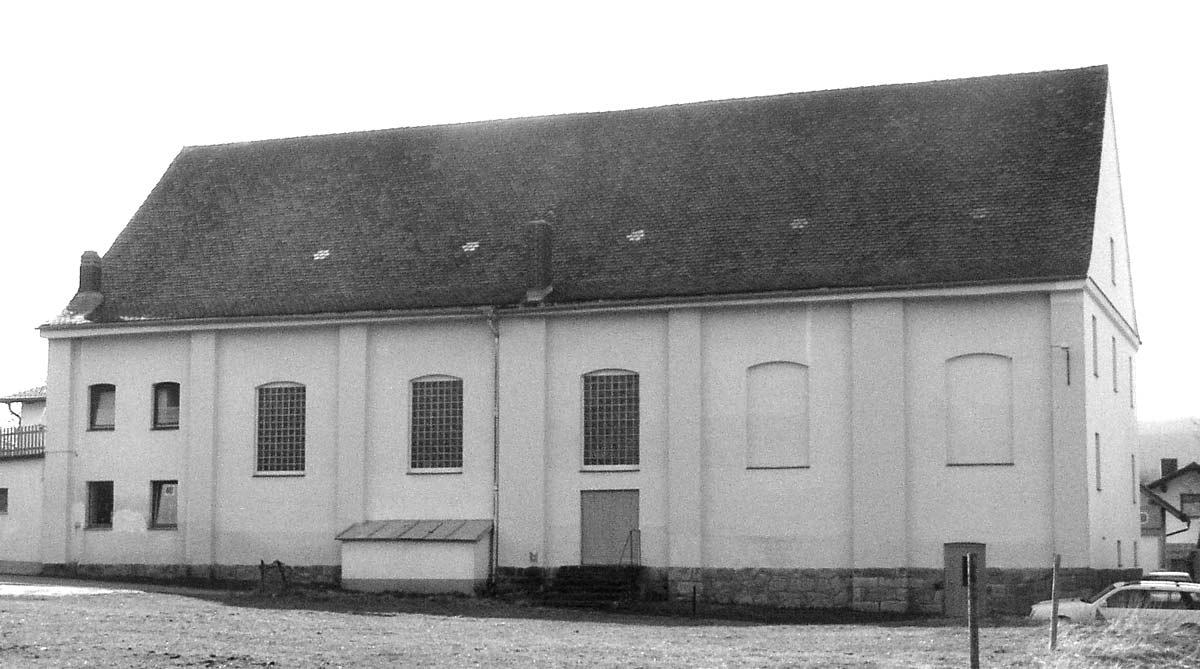
\includegraphics[width=9.303cm,height=5.168cm]{pictures/zulassungsarbeit-img023.jpg}

Abb. \stepcounter{Abb}{\theAbb}: Turnhalle des Turnvereins
Ruhmannsfelden\\
\end{supertabular}
\end{flushleft}
\end{minipage}
\end{center}
